\subsection{Scenario 1}

\subsubsection{Configuration}

Installer ettercap sur la machine :
\begin{minted}{bash}
$ sudo apt install ettercap-text-only
\end{minted}

Pour voir ce qui se passe au niveau du contrôleur, on pourra si on le souhaite lancer une session wireshark sur l'interface concernée afin d'examiner les divers paquets Openflow transitant entre ONOS et switchs (notamment les paquets ARP encapsulés en PACKET\_IN). Le filtre "tcp.port == 6633 \&\& openflow\_v4 \&\& openflow\_v4.type == OFPT\_PACKET\_IN" peut être utilisé pour supprimer les paquets inutiles.
Exécuter les instructions suivantes dans la console Mininet après avoir lancé le fichier general\_topology.py :

\begin{minted}{bash}
$ sudo ./general_topology.py [addresse IP du contrôleur]
$> h2 ping h11 &
$> h11 tcpdump -w scenario1/dump_victim.pcap -i h11-eth0 &
$> h6 ettercap -i h6-eth0 -T -w scenario1/dump_attacker.pcap -M ARP
/10.0.0.2// /10.0.0.11//
\end{minted}

Attendre quelques secondes que l'attaque se déroule, puis quitter ettercap avec "q" et quitter Mininet. 2 fichiers dans scenario1 (dump\_victim.pcap et dump\_attacker.pcap) doivent s'être rajoutés. Ils permettent de retracer l'attaque.

\subsubsection{Résultat}

Ouvrir le fichier dump\_attacker.pcap : on constate que h6 a bien intercepté le trafic entre h2 et h11.
Ouvrir le fichier dump\_victime.pcap : on constate que les pings proviennent et sont envoyés à l'adresse mac de h6 au lien de l'être à celle de h2.\\

\begin{figure}[h]
  	\centering
  	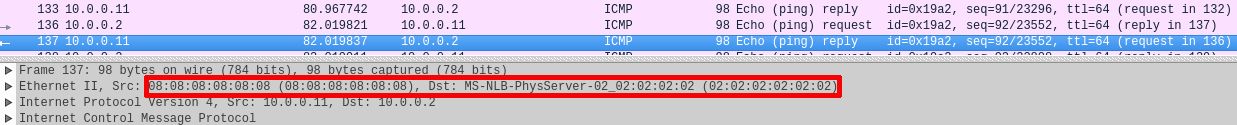
\includegraphics[width=1\textwidth]{ping_before.png}
  	\caption{Adresses ethernet concernées par le ping avant l'attaque : \url{08:08:08:08:08:08} et \url{02:02:02:02:02:02}}
\end{figure}

\begin{figure}[h]
  	\centering
  	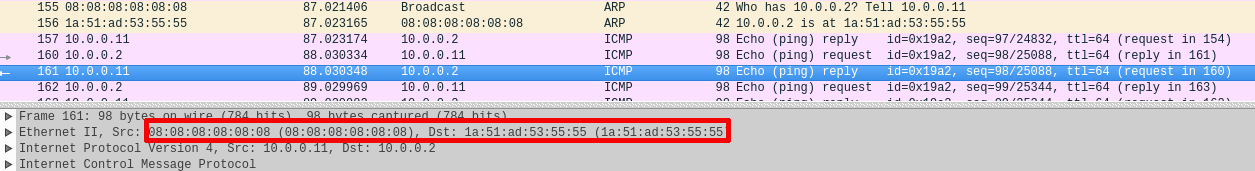
\includegraphics[width=1\textwidth]{ping_after.png}
  	\caption{Adresses ethernet concernées par le ping après l'attaque : \url{08:08:08:08:08:08} et \url{1a:51:ad:53:55:55}}
\end{figure}

Si wireshark a été utilisé au niveau du contrôleur, on peut constater les nombreux PACKET\_IN reçus encapsulant de l'ARP au début de l'attaque (h6 cherchant à obtenir les adresses mac de tous les équipements possibles sur le réseau (configurable dans ettercap, mais par défaut cela permet de repérer facilement l'attaque)).\\

\underline{Conclusion :}\\
Sans TLS activé au niveau de l'interface sud, il est possible d'agir fortement sur le réseau (action directe sur la topologie notamment). Avec TLS, il est toujours possible de modifier le trafic sur le plan de données à la volée. Il est possible d'empêcher cette attaque si le contrôleur intercepte et analyse tous les paquets ARP (attention au DoS éventuel dans ce cas).